\section{Informationstechnischer Aufbau}
\label{sec:Informationstechnischer Aufbau}




\subsection{Status Maschine}
\label{subsec:Status Maschine}

\begin{figure}[htb]
\centering		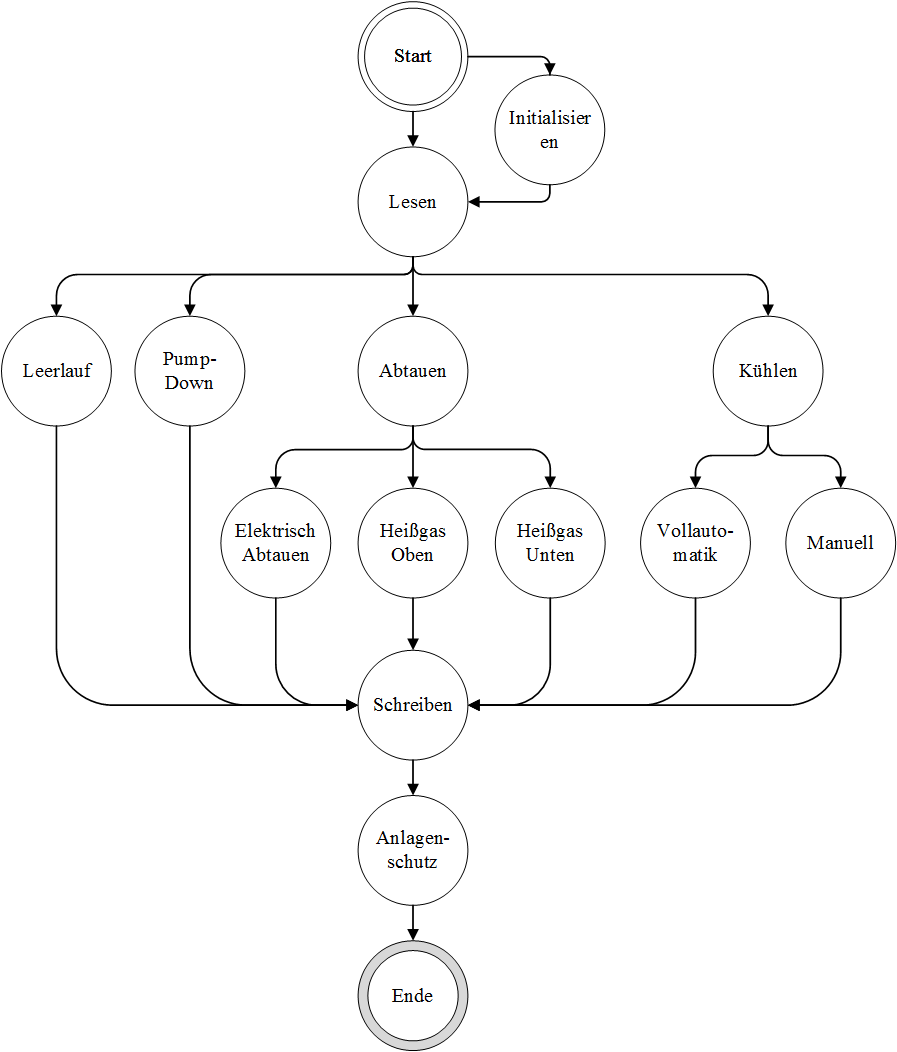
\includegraphics[width=0.90\textwidth]{Pictures/SM.png}
\caption{Status-Maschine}
\label{fig:SM}
\end{figure}

\subsection{Modbus RTU}
\label{subsec:Modbus RTU}

Beide Sensoren hatte eine fest eingestellte Stopbit-Größe. Der Drucktransmitter hat einen Stopbit, das Expansionsventil zwei.

\subsection{Grafical User Interface - GUI}
\label{subsec:GUI}


Drei Hauptzonen sind in der Abbildung farblich dargestellt. Das ist zum einen in \textit{grün} die Kompressor-Einheit. In der \textit{orange} Zone befinden sich der Verflüssiger und der Abtau-Verdampfer. Die \textit{blaue} Zone ist der Verdampfer, er befindet sich innerhalb der KK. Alle Komponenten außerhalb der blauen Zone sind außerhalb der KK installiert. 

 Im Kältekreislauf sind drei Wärmeübertrager installiert: In der \textit{organgenen} Zone sind zwei Wärmeübertrager dargestellt:

\subsection{Anlagenschutz}
\label{subsec: Anlagenschutz}